\documentclass[a4paper,11pt,fleqn]{article}%fleqn pour aligner les equations à gauche
\usepackage{/home/rweye/Documents/Overleaf/Styles/Cours}


\newcommand{\chnum}{Chapitre 6}
\newcommand{\chtitle}{Evolution spontanée d'un système chimique}
\newcommand{\dtype}{Cours}

\begin{document}
	\maketitle

\section{Transformations non totales}
	\subsection{Définition}
	Lors d'une transformation chimique \textbf{non totale}, aucun réactif n'est entièrement consommé. À l'état final, chacun des réactifs est donc encore présent et coexiste avec les produits, mais les quantités de matière de chaque espère n'évoluent plus. Un \textbf{état d'équilibre} est atteint.\\
	Expérimentalement, pour savoir si une transformation est totale ou non, il faut tester la présence de tous les réactifs et de tous les produits à l'état final.\\
	\textbf{Exemple :} Transformation non totale d'équation : \ce{Fe^2+(aq) + Ag+(aq) <--> Fe^3+(aq) + Ag(s)}\\
	\begin{tabular}{>{\centering}m{9cm} >{\centering\arraybackslash}m{9cm}}
	Composition du système à l'\textbf{état initial} & Composition du système à l'\textbf{état final} (ou état d'équilibre)\\
	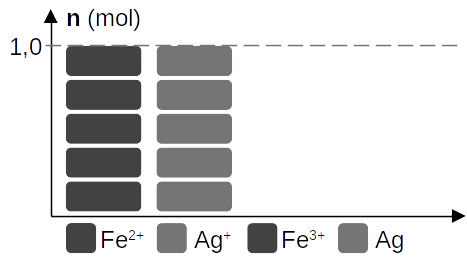
\includegraphics[scale=.4]{Ressources/TSPE_C7_Cours_Fig1.png} & 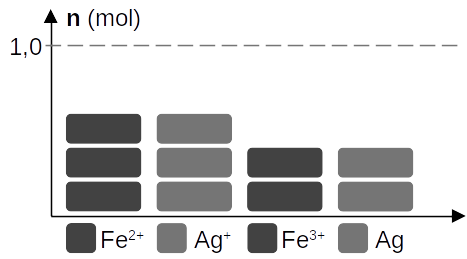
\includegraphics[scale=.4]{Ressources/TSPE_C7_Cours_Fig2.png}\\	
	\end{tabular}
	\subsection{Équilibre dynamique}
	Lors d'une transformation non totale, les réactifs réagissent entre eux pour former les produits et, simultanément, les produits réagissent entre eux pour former les réactifs. Lorsque les vitesses d'apparition et de disparition deviennent égales, un état d'équilibre est atteint : les quantités de matière de chaque espèce n'évoluent plus. Les deux réactions continuent néanmoins de se produire : on par le d'un \textbf{équilibre dynamique}.
	\textbf{Exemple :}\\
	\begin{tabular}{>{\centering}m{18cm}}
	\textbf{Sens direct}\\
	\schemestart
	\chemfig{Fe^{2+}_{(aq)} + Ag^{+}_{(aq)}}
	\arrow{->}
	\chemfig{Fe^{3+}_{(aq)} + Ag_{(s)}}
	\schemestop\\
	
\begin{tikzpicture}
\node (P) at (0,0) {\schemestart
	\chemfig{Fe^{2+}_{(aq)} + Ag^{+}_{(aq)}}
	\schemestop};
\node (S) at (6,0) {\schemestart
	\chemfig{Fe^{3+}_{(aq)} + Ag_{(s)}}
	\schemestop};
\node (L) at (3,0) {\schemestart
	\arrow{<=>}
	\schemestop};
\draw[->,>=latex] (P) to[bend left] (S);
%\draw[->,>=latex] (L) to[bend left] (S);
\draw[->,>=latex] (S) to[bend left] (P);
\end{tikzpicture}\\
	
	\schemestart
	\chemfig{Fe^{3+}_{(aq)} + Ag_{(s)}}
	\arrow{->}
	\chemfig{Fe^{2+}_{(aq)} + Ag^{+}_{(aq)}}
	\schemestop\\
	\textbf{Sens indirect}\\	
	\end{tabular}\\
	Pour tenir compte du fait que la \textbf{transformation chimique s'effectue dans les deux sens} (appelés sens direct et sens indirect), l'équation de la réaction s'écrit avec une \textbf{double flèche} \ce{<=>}.
	
	\subsection{Taux d'avancement final}
	Le \textbf{taux d'avancement final} d'une transformation, noté $\tau$ (tau), est le rapport entre l'avancement final ($x_f$) et l'avancement maximal ($x_{max}$). On a :
	$$\tau = \frac{x_f}{x_{max}}$$
	Si $\tau = 1$ la transformation est totale ($x_f = x_{max}$)\\
	Si $\tau < 1$ la transformation est non totale ($x_f < x_{max}$)

\section{Évolution spontanée d'un système}
On peut déterminer le sens dans lequel une transformation se produit spontanément à l'aide de son quotient de réaction.
	\subsection{Quotient de réaction $Q$}
	Pour une transformation chimique en solution aqueuse d'équation : \ce{aA(aq) + bB(aq) <=> cC(aq) + dD(aq)}, le quotient de réaction a pour expression :
	$$Q_r = \dfrac{\left( \dfrac{[C]}{c^0}\right)^c \times \left( \dfrac{[D]}{c^0}\right)^d}{\left( \dfrac{[A]}{c^0}\right)^a \times \left( \dfrac{[B]}{c^0}\right)^b}$$
	Remarques :
	\begin{itemize*}
		\item les espèces solides n'interviennent pas dans cette expression
		\item l'eau, en tant que solvant, n'intervient pas dans cette expression, même si elle figure dans l'équation de la réaction
	\end{itemize*}
	\textbf{Exemple : Donner l'expression du quotient de réaction pour la transformation suivante :}
	\vspace*{2cm}
	
	\subsection{Constante d'équilibre $K$}
	Lorsque le système atteint un état d'équilibre, le quotient de réaction $Q_{r,éq}$ est appelé \textbf{constante d'équilibre} et est  noté $K$. Ainsi $Q_{r,éq} = K$. Cette grandeur ne dépend pas de la composition initiale du système. Elle dépend uniquement de la température.\\
	Si la constante d'équilibre est très grande ($K>10^4$), la transformation est considérée comme totale.
	
	\subsection{Sens d'évolution spontanée}
	Tout système évolue spontanément vers un état d'équilibre. Son quotient de réaction tend alors vers la constante d'équilibre. On peut donc prévoir le \textbf{sens d'évolution spontanée} d'un système en \textbf{comparant} les valeurs du quotient de réaction à l'état initial $Q_{r,i}$ et la constante d'équilibre $K$.
\newpage
\section{Transfert spontané d'électron}
	\subsection{Réaction d'oxydo-réduction}
	\subsubsection*{Rappels :}
	\begin{tabular}{>{\centering}m{.5\textwidth} | >{\centering\arraybackslash}m{.5\textwidth}}
	\textbf{Demi-équation électronique} & \textbf{Équation d'oxydoréduction}\\
	$\xrightarrow{\text{\large{Réduction}}}$ & \fbox{$2 \times$} \ce{Al(s) <=> Al^3+(aq) + 3 e-}\\
	
	Oxydant \hspace{.5cm} \ce{Ox + n e- <=> Red} \hspace{.5cm} Réducteur &\fbox{$3 \times$} \ce{Cu^2+(aq) + 2 e- <=> Cu(s)}\\
	$\xleftarrow{\text{\large{Oxydation}}}$ & \ce{2 Al(s) + 3 Cu^2+(aq) -> 2 Al^3+(aq) + 3 Cu(s)} \\
	\end{tabular}\\
	
	Lors d'une réaction d'oxydoréduction, un \textbf{transfert spontané d'électrons} se produit entre les réactifs :
	
	\begin{tabular}{m{.7\textwidth}m{.3\textwidth}}
	- directement si les réactifs sont en contact &
		\begin{tikzpicture}
			\node[draw,circle,fill = gray!50] (Zn) at (0,0) {\textbf{\ce{Zn}}};
			\node[draw,circle,fill = gray!50] (Cu) at (1.1,-.25) {\textbf{\ce{Cu^2+}}};
			\node (e) at (.6,.4) {\textbf{\ce{e-}}};
			\draw[-latex] (0.2,.2) edge[bend left] (1,0);
		 \end{tikzpicture}\\
	 - indirectement, par l'intermédiaire d'un circuit extérieur si les réactifs ne sont pas en contact&
		\begin{tikzpicture}
			\node[draw,circle,fill = gray!50] (Zn) at (0,0) {\textbf{\ce{Zn}}};
			\node[draw,circle,fill = gray!50] (Cu) at (2,0) {\textbf{\ce{Cu^2+}}};
			\node (e) at (1,.4) {\textbf{\ce{e-}}};
			\draw[fill=orange!20] (0.3,-.15)--(0.3,.15)--(1.5,.15)--(1.5,-.15)--cycle;
			\draw[-stealth] (.4,0) to (1.4,0);
			\node (circ) at (1,-.8) {\textbf{Circuit}};
			\draw[-stealth,thin] (1,-.7)--(1,-.15);
		 \end{tikzpicture}\\
	\end{tabular}
	\subsubsection*{Oxydants et réducteurs usuels}
	\begin{tabular}{|>{\centering}m{.3\textwidth} |>{\centering}m{.3\textwidth} |  >{\centering\arraybackslash}m{.3\textwidth}|}
	\hline \textbf{Espèce chimique} & \textbf{Caractère} & \textbf{Exemples d'utilisation}\\
	\hline Ion hypochlorite \ce{ClO-} & Oxydant & Eau de Javel\\
	\hline Dichlore \ce{Cl2} & Oxydant & Production d'acide chlorhydrique\\
	\hline Dioxygène \ce{O2} & Oxydant & Air, Pile à combustible\\
	\hline Dihydrogène \ce{H2} & Réducteur & Pile à combustible\\
	\hline Acide ascorbique (vitamine C) & Réducteur & Anti-oxydant dans l'alimentation\\
	\hline Métaux du bloc s (lithium, magnésium) & Réducteur & Piles et batteries\\
	\hline
	\end{tabular}\\
	
	Les métaux du bloc s (colonnes 1 et 2 du tableau périodique) sont de très bons réducteurs car ils perdent très facilement 1 ou 2 électrons pour atteindre la configuration électronique de valence du gaz noble le plus proche.
	\textbf{Exemples : Lithium et Magnésium}	 \vspace{3cm}
	\subsection{Piles électrochimiques}
	
	\subsubsection*{Principe :}
	Une pile génère un courant électrique, c'est-à-dire une circulation de charges, à partir d'une \textbf{réaction d'oxydo-réduction spontanée}. Elle convertit ainsi de l'énergie chimique en énergie électrique.
	
	\subsubsection*{Constitution et fonctionnement :}
	Une \textbf{pile} est constituée de deux compartiments distincts, appelés \textbf{demi-piles}, séparés par un \textbf{pont salin} ou une \textbf{membrane}.
	\begin{itemize}
		\item Chaque \textbf{demi-pile} est constitué d'un solide conducteur appelé \textbf{électrode}, plongeant dans un milieu ionique.
		\item Chaque demi-pile contient un \textbf{couple oxydant/réducteur}:
		\begin{itemize}
			\item l'une est le siège d'une \textbf{oxydation} : des électrons sont produits : ils alimentent ensuite le circuit extérieur
			\item l'autre est le siège d'une \textbf{réduction} : les électrons ayant circulé dans le circuit sont récupérés.
		\end{itemize}
		Les demi-piles sont séparées par un \textbf{pont salin} ou une \textbf{membrane}. Ce séparateur :
		\begin{itemize}
			\item empêche le contact direct entre les espèces chimiques de chaque demi-pile et oblige ainsi à un transfert indirect par un circuit extérieur
			\item permet d'assurer la neutralité électrique des milieux ioniques par migration d'ions spectateurs
		\end{itemize}
	\end{itemize}
	La circulation  d'électrons à l'extérieur de la pile et d'ions à l'intérieur de la pile constituent le \textbf{courant électrique}. Par convention, le courant circule dans le sens inverse des électrons.
	
	\begin{figure}[h!]
    \centering
    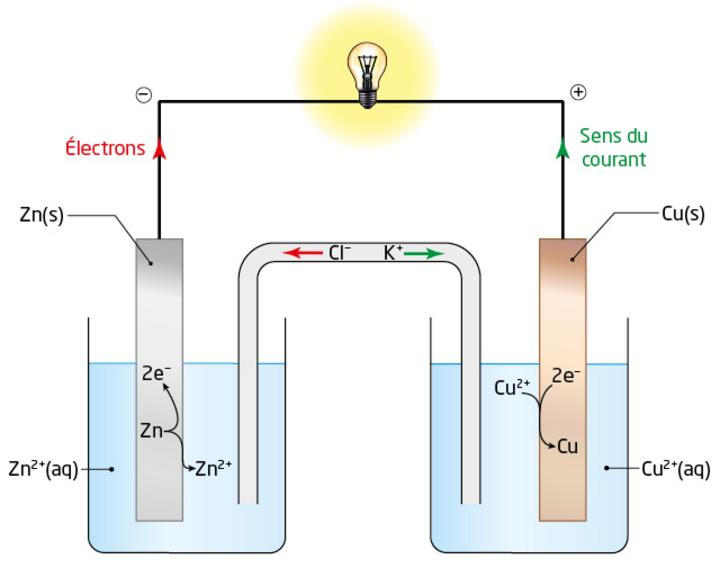
\includegraphics[scale=.45]{Ressources/TSPE_C16_Cours_Fig1.png}
    \caption*{\textbf{Schéma de la pile}}
     \end{figure}
     
	\subsubsection*{Tension à vide et polarité :}
	La \textbf{tension à vide} d'une pile est la valeur absolue de la tension entre ses électrodes en circuit ouvert. Elle dépend des couples oxydant/réducteur mis en jeu, des concentrations en ions et de la température.\\
	La tension à vide se mesure en branchant un voltmètre aux bornes de la pile. Cette mesure permet de déterminer la \textbf{polarité des électrodes}. Si la tension mesurée est positive, on a :\\
	\begin{tabular}{|>{\centering}m{2.5cm}|>{\centering}m{2.5cm}|>{\centering}m{2.5cm}|>{\centering\arraybackslash}c}
	\cline{1-3} Voltmètre & Borne V & Borne COM & \multirow{2}{*}{ 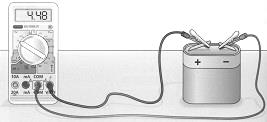
\includegraphics[scale=.6]{Ressources/TSPE_C16_Cours_Fig2.png}}\\
	\cline{1-3} Pile & + & - &\\
	\cline{1-3}	
	\end{tabular}
	\newpage
	\subsubsection*{Usure :}
	Une pile en fonctionnement est un système chimique qui évolue spontanément vers un état d'équilibre ($Q_r$ tend vers $K$). Lorsque cet \textbf{état d'équilibre} est atteint ($Q_r = K$), la pile est usée : elle ne débite plus de courant. L'usure d'une pile peut aussi survenir avant que $Q_r$ n'atteigne $K$ si un des réactif est totalement consommé (la transformation est totale dans ce cas).\\
	\subsubsection*{Capacité électrique :}
	Pour adapter une pile à un usage souhaité il convient d'évaluer sa \textbf{capacité électrique}, c'est-à-dire la charge électrique maximale $q_{pile}$ qu'elle peut fournir durant toute sa durée de vie. Elle peut être calculée par la relation :\\
	\begin{tabular}{>{\centering}m{5cm} | >{\arraybackslash}l}
	& $q_{pile}$ en coulomb (\unit{\coulomb})\\
	& $n_{\ce{e-},ech,max}$ : quantité maximale d'électrons échangés en mole (\unit{\mole})\\
	$q_{pile}=n_{\ce{e-},ech,max} \times N_A \times e$ & $N_A$ : constante d'Avogadro ($N_A \approx$ \num{6,02e23} \unit{\per \mole})\\
	$=n_{\ce{e-},ech,max} \times \mathcal{F}$& $e$ : charge élémentaire ($e \approx$ \num{1,60e-19} \unit{\coulomb})\\
	& $\mathcal{F}$ : constante de Faraday ($\mathcal{F} \approx$ \num{96,5e3} \unit{\coulomb \per \mole})\\
	\end{tabular}\\
	
	\underline{Remarque 1} : La charge électronique d'une pile  est parfois notée $Q_{pile}$ ou $Q_{max}$ à ne pas confondre avec le quotient de réaction !\\
	La capacité électrique d'une pile se détermine à partir de la quantité initiale de réactif limitant et de la réaction électrochimique.\\
	Exemple : Une pile cuivre-zinc contient \num{0,20} \unit{\mole} de zinc. On suppose que le zinc est le réactif limitant.
	\vspace{3cm}
	
	\underline{Remarque 2} : Dans le commerce, la capacité électrique des pile est estimée en \unit{\milli\ampere\hour} car elle dépend de l'intensité du courant délivré et de la durée de fonctionnement : $q_{pile} = I \times \Delta t$.\\
	\begin{tabular}{|l|l|}
	\hline \num{1} \unit{\coulomb} & \num{1} \unit{\ampere \cdot \second}\\
	\hline \num{3600} \unit{\coulomb}& \num{1} \unit{\ampere \cdot \hour}\\
	\hline
	\end{tabular}
\end{document}